% !TeX spellcheck = en_EN-English
\documentclass[a4paper]{article}
\usepackage[slovak]{babel}
\usepackage[utf8]{inputenc}
\usepackage[T1]{fontenc}
\usepackage{a4wide}
\usepackage{amsmath}
\usepackage{amsfonts}
\usepackage{amssymb}
\usepackage{mathrsfs}
\usepackage[small,bf]{caption}
\usepackage{subcaption}
\usepackage{xcolor}
\usepackage{graphicx}
\usepackage{enumerate}
\usepackage{hyperref}



\pagestyle{empty}
\setlength{\parindent}{0pt}

\newenvironment{modenumerate}
{\enumerate\setupmodenumerate}
{\endenumerate}

\newif\ifmoditem
\newcommand{\setupmodenumerate}{%
	\global\moditemfalse
	\let\origmakelabel\makelabel
	\def\moditem##1{\global\moditemtrue\def\mesymbol{##1}\item}%
	\def\makelabel##1{%
		\origmakelabel{##1\ifmoditem\rlap{\mesymbol}\fi\enspace}%
		\global\moditemfalse}%
}

\renewcommand{\thesubsection}{\alph{subsection})}

\makeatletter
\def\@seccntformat#1{%
	\expandafter\ifx\csname c@#1\endcsname\c@section\else
	\csname the#1\endcsname\quad
	\fi}
\makeatother

\begin{document} 
	
	\pagenumbering{arabic}
	\pagestyle{plain}
	
	\begin{center}
		\sc\large
		MBI Homework 2 for CS students
	\end{center}
	
	Autor: Marián Kravec
	
	\subsection{}
	
	Firstly we implement functions that get two bases and time, and returns probability that first base change to second in that time based on Jukes-Cantor model:
	
	\centerline{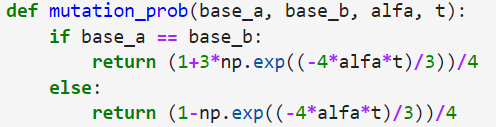
\includegraphics[width=0.5\textwidth]{mut_prob}} 
	
	Now we can implement Falsenstein's algorithm (I am not sure whether my implementation can be considered as dynamical programming or it's recursive with memoization but results are equal):
	
	\centerline{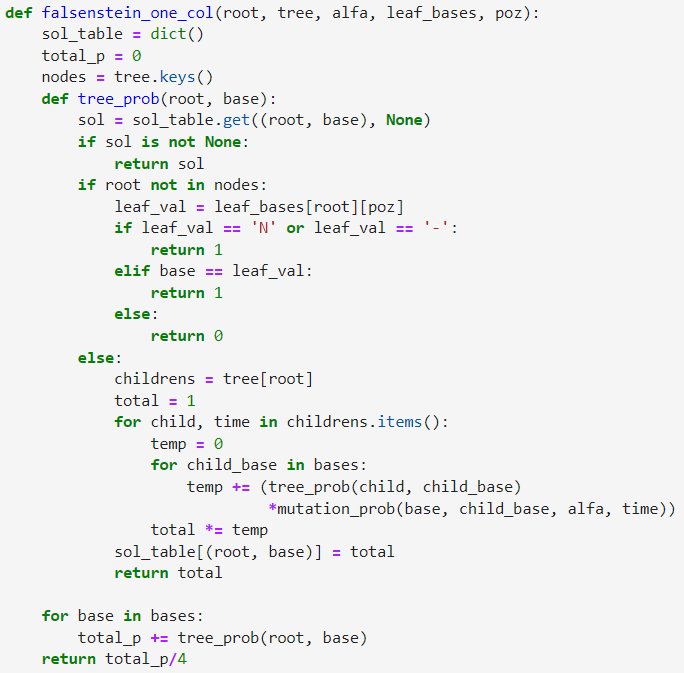
\includegraphics[width=0.9\textwidth]{falsenstein}} 
	
	\newpage
	\subsection{}
	
	If we run this algorithm on tree stored in tree.txt, setting all leaf bases to $A$ and setting mutation speed to $\alpha = 1$ and $\alpha = 0.2$ we get these values:

	\begin{table}[!h]
		\begin{tabular}{|l|l|l|}
			\hline
			$\alpha$ & probability (float) & probability (percentage)\\ \hline
			1 & 0.054 & 5.4\% \\ \hline
			0.2 & 0.183 & 18.3\% \\ \hline
		\end{tabular}
	\end{table}
	(I got bit confused by information in assignment "The probability of each base in the equilibrium is $\frac{1}{4}$, which is used as probability $q_a$ of generating base a in the root" whether this information means that information means that I need to divide probability in root by four or not, after discussion with some classmates I did exactly that (divide by four) and got values in table above instead of values $21.8\%$ for $\alpha=1$ and $73.3\%$ for $\alpha=0.2$)
	\\
	\\
	We can see that smaller mutation speed resulted in higher probability. This makes sense because fact that all bases are same means either that no mutations happened or that mutations happened but also 'inverse' mutations happened that returned bases back to initial state. Out of these two cases no mutations is more likely scenario however likelihood of this scenario decrease as mutation speed increase but probability to not change decrease.
	
	\subsection{}
	
	Now we implement function that can give us probability of whose sequence rather that one column. This function compute probability for each column and because we expect that columns are independent we multiply those values (to not have issues with very small numbers we sum logarithms of probabilities for columns and in the end we compute it back to probability value by putting it as exponent).
	
	\centerline{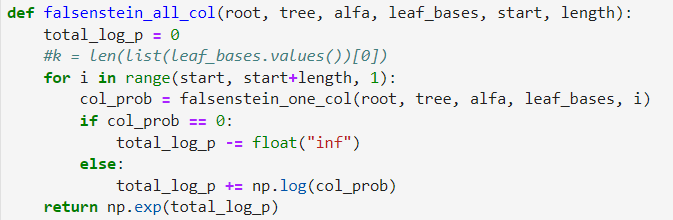
\includegraphics[width=0.8\textwidth]{falsenstein_2}} 
	
	We also implement function that run Falsenstein's algorithm on inputted tree for 20 values of mutation speed $\alpha$ (between 0.1 to 2 with step 0.1) and return one for which Falsenstein's algorithm returned highest probability.
	
	\centerline{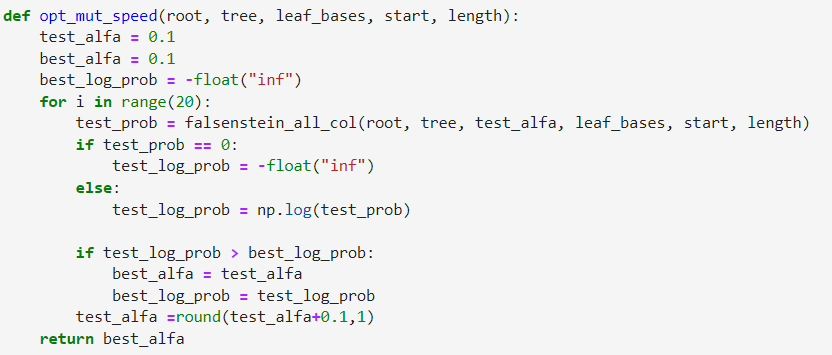
\includegraphics[width=1\textwidth]{opt_alfa}} 
	
	\subsection{}
	
	Now we will read file cftr.txt which contains aligned sequences for animals in leafs of our tree. Now we will split this sequences into non-overlapping windows with size 100 and for each window we compute most likely value of mutation speed $\alpha$ using function we implemented in previous section. 
	
	For first 10 windows we get these values $\alpha*$: 
	
	\begin{table}[!h]
		\begin{tabular}{|l|l|}
			\hline
			position  & $\alpha*$\\ \hline
			1-100 & 1.0  \\ \hline
			201-200 & 1.2  \\ \hline
			301-300 & 1.1  \\ \hline
			401-400 & 2.0  \\ \hline
			501-500 & 1.6  \\ \hline
			601-600 & 1.0  \\ \hline
			701-700 & 1.5  \\ \hline
			801-800 & 1.3  \\ \hline
			901-1000 & 2.0  \\ \hline
			1001-1100 & 1.1  \\ \hline
		\end{tabular}
	\end{table}
	
	\subsection{}
	
	After we compute $\alpha*$ for all windows we split them into groups that contain at least one base from exons and into those that are contain only bases from introns (for that we will use file exons.txt). After split we can visualize their distribution using histogram (we used density view of histogram for better comparison because windows that have overlap with exon are only small fraction of all windows):
	
	\centerline{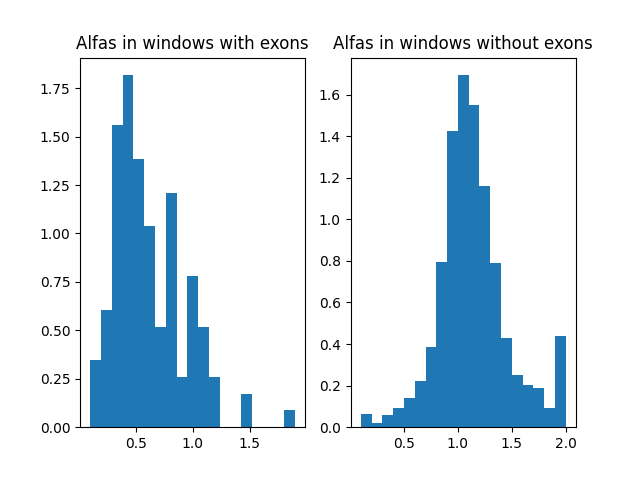
\includegraphics[width=1\textwidth]{exons_non_exons_comp.png}} 
	
	We can see that their distribution is quite different. Let's put them both into one histogram for better comparison:
	
	\centerline{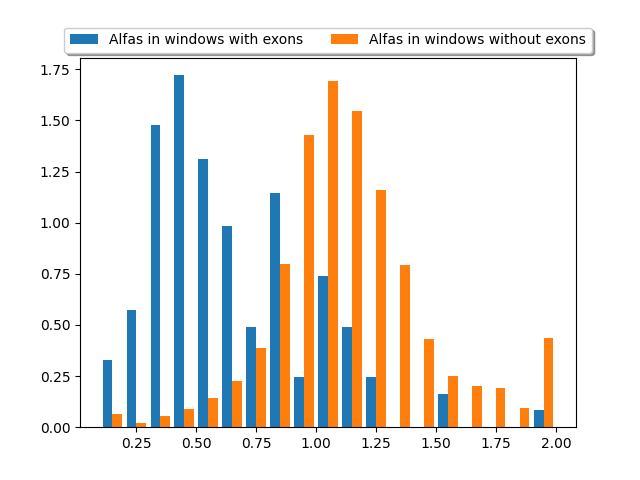
\includegraphics[width=1\textwidth]{exons_non_exons_comb.png}} 
	
	In this histogram we can clearly see difference. We can see that optimal value $\alpha$ for windows that contains at least one base from exon is generally smaller than optimal value for windows containing only intron. This is expected because lower mutation speed means that there are less mutations in given time and mutation in exons are much more dangerous then in introns. It's more dangerous because exons are parts of genome that gets translated into protein and change in one base means change in codon which could mean change in amino acid which could change structure and functionality of resulting protein. On the other hand changes in introns have smaller consequences and because of that their mutation speed can be higher so mutations in them are more frequent. 
\end{document}
